\documentclass{article}

\usepackage{amsmath}
\usepackage{amssymb}
\usepackage{amsfonts}
\usepackage{parskip}
\usepackage{fullpage}
\usepackage{hyperref}
\usepackage{tikz}
\usepackage{url}
\usepackage{subfig}
\usepackage[backend=bibtex]{biblatex}

\usepackage{bettelini}

\hypersetup{
    colorlinks=true,
    linkcolor=black,
    urlcolor=blue,
    pdftitle={Improved bead sort using the Fourier Transform},
    pdfpagemode=FullScreen,
}

\addbibresource{./references.bib}

\title{Improved bead sort using the Fourier Transform}
\author{Paolo Bettelini}
\date{\today}

\begin{document}

\maketitle

\section{Introduction}

\subsection{Abstract}

Bead sort has always been an interesting, but useless, sorting algorithm
for integers. It is able to sort numbers without ever directly comparing them.
This paper presents an attempt to make it possibly more efficient
for software when sorting large arrays of numbers.
The resulting algorithm is more efficient (less than \(O(N^2)\)) when sorting a large array of small integers,
preferably with few distinct elements.

\subsection{Bead sort}

\textit{Bead sort}\cite{beadsort} or \textit{gravity sort}
is a natural sorting algorithm.
This algorithm is primarily used to sort
integers, but can be extended to sort the rationals.

The basic idea is to represent the unsorted integers
in a matrix (\ref{fig:a}), where each columns has \(n\) beads.
We then shift every bead to the right side of the matrix
until they collide with another bead,
as if they were affected by gravity.
The final step is to count the elements in each columns,
forming the final ordered sequence (\ref{fig:b}).

\begin{figure}[h]
    \centering
  
    \subfloat[Unsorted beads]{
        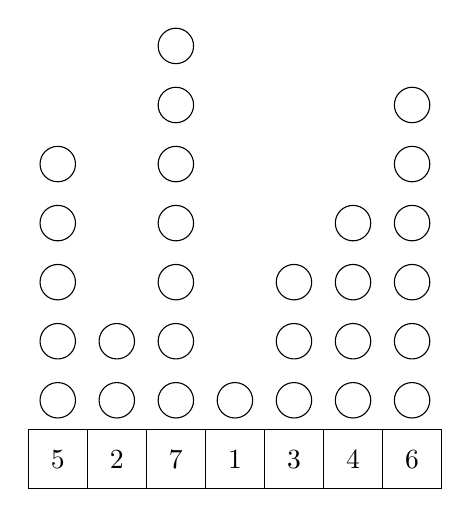
\begin{tikzpicture}[scale=0.75]
            % Draw the array
            \foreach \i/\n in {0/5, 1/2, 2/7, 3/1, 4/3, 5/4, 6/6} {
                \draw (\i,0) rectangle ++(1,1);
                \node at (\i+0.5, 0.5) {\n};
            }
            
            % Beads
            \foreach \i/\n in {0/5, 1/2, 2/7, 3/1, 4/3, 5/4, 6/6} {
                \pgfmathsetmacro{\beads}{\n}
                \foreach \j in {1,...,\beads} {
                \draw (\i+0.5, \j+0.5) circle (0.3cm);
                }
            }
        \end{tikzpicture}
        \label{fig:a}
    }
    \quad\(\longrightarrow\)\quad
    \subfloat[Sorted beads]{
        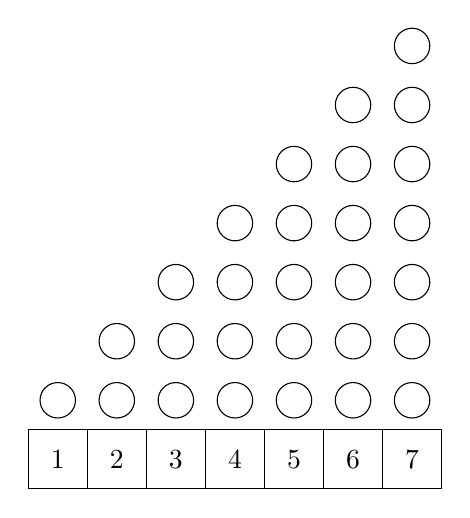
\begin{tikzpicture}[scale=0.75]
            % Draw the array
            \foreach \i/\n in {0/1, 1/2, 2/3, 3/4, 4/5, 5/6, 6/7} {
                \draw (\i,0) rectangle ++(1,1);
                \node at (\i+0.5, 0.5) {\n};
            }
            
            % Beads
            \foreach \i/\n in {0/1, 1/2, 2/3, 3/4, 4/5, 5/6, 6/7} {
                \pgfmathsetmacro{\beads}{\n}
                \foreach \j in {1,...,\beads} {
                \draw (\i+0.5, \j+0.5) circle (0.3cm);
                }
            }
        \end{tikzpicture}
        \label{fig:b}
    }
  
    \caption{Beads matrix for \(S = 5,2,7,1,3,4,6\)}
    \label{fig:both}
\end{figure}

The time complexity of this algorithm, depending on the implementation, ranges from \(O(1)\)
to \(O(P)\) where \(P=\sum S_k\).

\pagebreak

\section{Algorithm}

\subsection{Core idea}

Let \(S\) be the list of unsorted positive integers.

The core idea is to represents the beads matrix as a
sum of sine functions. Each frequency represents a row of beads,
and its amplitude the amount of elements in it.

\textbf{Example for \(S = 5,3,5,6,1,2\):}

\begin{minipage}{0.3\textwidth}
    \begin{flushright}        
    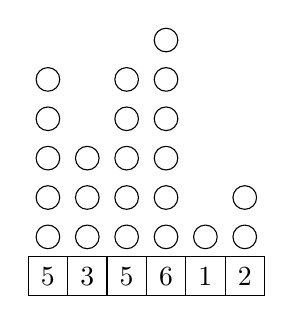
\begin{tikzpicture}[scale=0.5]
        % Draw the array
        \foreach \i/\n in {0/5, 1/3, 2/5, 3/6, 4/1, 5/2} {
            \draw (\i,0) rectangle ++(1,1);
            \node at (\i+0.5, 0.5) {\n};
        }
        
        % Beads
        \foreach \i/\n in {0/5, 1/3, 2/5, 3/6, 4/1, 5/2} {
            \pgfmathsetmacro{\beads}{\n}
            \foreach \j in {1,...,\beads} {
                \draw (\i+0.5, \j+0.5) circle (0.3cm);
            }
        }
    \end{tikzpicture}
    \end{flushright}
\end{minipage}
\begin{minipage}{0.5\textwidth}
    \[
        6\sin(t) + 5\sin(2t) + 4\sin(3t) + 3\sin(4t)+3\sin(5t)+\sin(6t)
    \]
\end{minipage}

We define this function as a time-dependent function \(X_S(t)\).
\[
    X_S(t) \triangleq
    \sum_{k=1}^{|S|}
    \sum_{f=1}^{n_k}
    \sin(ft)
\]

By using the Fourier Transform on the function representing the matrix
we can retrieve the amplitudes of the different frequencies
and represent the final beads matrix.
Thus, we get a frequency-dependent function
\[
    \hat{X}_S(\xi)
    \triangleq
    \mathcal{F}\{X_S(t)\}
\]

For all \(\xi \in \mathbb{N}\), the frequencies given by
\(|\hat{X}_S(\xi)|\) are integers, and they follow the property
\(|\hat{X}_S(\xi)| \geq |\hat{X}_S(\xi+1)|\).
The first is value is \(|\hat{X}_S(1)|=|S|\) since every number in \(S\) produces 
the frequency 1 of the first row of beads (every element is at least 1). \\
In order to retrieve the ordered elements, we can gradually increase
the frequency \(\xi\) by \(1\) starting at \(\xi=1\). \\
Let \(k=|\hat{X}_S(\xi)| - |\hat{X}_S(\xi+1)|\). Whenever \(k \neq 0\)
we consider \(\xi\) to be the next elements in the list of ordered
integers. The element \(\xi\) will be the next in the ordered sequence,
and it will appear \(k\) many times.
Repeat this process until all numbers have been extracted
(\(\xi = \text{max}(S)\) or \(|\hat{X}_S(\xi)|=0\)).

\textbf{Example for \(S = 5,3,5,6,1,2\):}
The first values of \(|\hat{X}_S(\xi)|\) for positive integer frequencies are the following
\[
    6, 5, 4, 3, 3, 1, 0, 0, 0, 0, \cdots
\]
We are looking for the case where \(k \neq 0\), meaning whenever
\(|\hat{X}_S(\xi+1)| < |\hat{X}_S(\xi)|\). \\
At position \(1\), the value \(6\) decreases to \(5\), meaning that the first sorted element is \(1\). \\
At position \(2\), the value \(5\) decreases to \(4\), meaning that the next sorted element is \(2\). \\
At position \(3\), the value \(4\) decreases to \(3\), meaning that the next sorted element is \(3\). \\
At position \(5\), the value \(3\) decreases to \(1\), meaning that the next sorted elements are the number \(5\)
repeated two times (\(3-1=2\)). \\
At position \(6\), the value \(1\) decreases to \(1\), meaning that the last sorted element is \(6\).

It is important to note that the duplicate numbers,
such as \(5\) in this case, collapse under the same
point in \(|\hat{X}_S(\xi)|\).

\pagebreak

\subsection{Computation}

\subsubsection{Complexity of \(X_S(t)\)}

The function \(X_S(t)\) has time complexity \(O(N\cdot P)\) where
\(P=\sum S_k\).
This is because we need to add a term for each bead in the matrix.
We can reduce the latter by noting that \(X_S(t)\) contains
a geometric series.

\begin{align*}
    \sum_{f=1}^{n_k} \sin(ft) 
    &= \Im \sum_{f=1}^{n_k} e^{ift} \\
    &= \Im \left( e^{it} \frac{e^{itn_k}-1}{e^{it}-1} \right) \\
    &= \Im \left( e^{it} \frac{e^{in_kt/2}(e^{in_kt/2} - e^{-in_kt/2})}
        {e^{it/2}(e^{it/2} - e^{-it/2})} \right) \\
    &= \Im \left( e^{it} \frac{e^{in_kt/2}(2i\sin(n_kt/2))}
        {e^{it} (2i\sin(t/2))} \right) \\
    &= \Im \left( e^{i(n_k+1)t/2} \frac{\sin(n_k t/2)}{\sin(t/2)} \right) \\
    &= \Im \left(
            ( \cos((n_k+1)t/2) + i\sin((n_k+1)t/2)) \frac{\sin(n_k t/2)}{\sin(t/2)}
        \right) \\
    &= \frac{\sin(n_k t/2)}{\sin(t/2)} \sin((n_k+1)t/2)
\end{align*}

Thus,
\[
    X(t) = \sum_{k=1}^{|S|} \frac{\sin(n_k t/2)}{\sin(t/2)} \sin((n_k+1)t/2)
\]
The time complexity of \(X_S(t)\) is now \(O(N)\).

\subsubsection{Complexity of \(\hat{X}_S(\xi)\)}

One approach to compute the values of \(\hat{X}_S(\xi)\) would be to use the
FFT algorithm. The time complexity of the FFT is \(O(N\log(N))\), but we would first
need to allocate a discrete approximation of \(X_S(t)\) in memory.
This procedure would need to allocate \(\text{max}(S)\) values, resulting in a space complexity
of \(O(\text{max}(S))\). Furthermore, computing a value of \(X_S(t)\) has time complexity
\(O(N^2)\), meaning that this operation would have time complexity \(O(N^2) + O(N\log(N)=O(N^2))\).
This would also be the total time complexity of the algorithm, since the
retrieval of sorted integers is at most \(O(N)\)
(using a linear scan of the frequencies, which are already allocated in memory).

Another approach is to use an approximation to a closed-form of \(\hat{X}_S(\xi)\). \\
The Fourier Transform of \(X_S(t)\) is given by
\begin{align*}
    \hat{X}_S(\xi) &=
    \frac{1}{\text{max}(S)-1}
    \integral[1][\text{max}(S)]
    [e^{-2\pi it\xi}X(t)] [t] \\
    &= \frac{1}{\text{max}(S)-1}
    \integral[1][\text{max}(S)]
    [e^{-2\pi it\xi}\sum_{k=1}^{|S|} \frac{\sin(n_k t/2)}{\sin(t/2)} \sin((n_k+1)t/2)]
    [t]
    \\ 
\end{align*}

Since \(|S|\) is finite we can apply an
interchange of summation and integration
\[
    \hat{X}_S(\xi) =
    \frac{1}{\text{max}(S)-1}
    \sum_{k=1}^{|S|}
    \,
    \integral[1][\text{max}(S)]
    [\frac{\sin(n_k t/2)}{\sin(t/2)} \sin((n_k+1)t/2)e^{-2\pi it\xi}]
    [t]
\]

The space complexity of this approach would be \(O(1)\). As a side effect,
the values of \(\hat{X}_S(\xi)\) are not allocated, so their computation
has always time complexity of \(O(N)\).

\subsubsection{Complexity of the retrieval}

The ordered elements need to be retrived from \(\text{max}(S)\) values of
\(\hat{X}_S(\xi)\). Let \(A\) be the average distance between two consecutive sorted
elements in \(S\) and \(D\) be the amount of distinct elements in \(S\).\\
Note that \(D \cdot A \approx \text{max}(S)\).
\\
Considering a closed-form for \(\hat{X}_S\), the retrival has time complexity
\(O(N^2)\) if we linearly scan the frequencies given by \(|\hat{X}_S|\).

We can optimize this operation by using a sort of binary search.
The binary search will be used to reach the next point where \(|\hat{X}_S|\) decreases.
The binary search will be repeated \(D\) times, and for each time
it will travel approximately \(A\) values. Since computing each value has cost \(O(N)\),
and the cost of a binary search is \(O(\log(N))\),
the final time complexity is \(O(D\cdot N \log(A))\).

\section{Conclusion}

In conclusion we have the following complexities: \\
\textbf{FFT}
\begin{itemize}
    \item \text{Time complexity:} \(O(N^2)\)
    \item \text{Space complexity:} \(O(\text{max}(S))\)
\end{itemize}
\textbf{Closed-form}
\begin{itemize}
    \item \text{Time complexity:} \(O(D\cdot N \log_2(A))\)
    \item \text{Space complexity:} \(O(1)\)
\end{itemize}

The latter time complexity is generally more than \(O(N^2)\),
but as \(N \to \infty\), with smaller values for \(D\) and \(A\) it may actually
be a good compromise.

For both of the implementations the complexities are independant
of the initial order status of \(S\).

\nocite{*} % cite all entries

\printbibliography

\end{document}
